\chapter{Marco Teórico} \label{chap:marcoteorico}

En el siguiente capitulo se pondrá al alcance del lector las bases teóricas y los conocimientos necesarios para poder entender las diferentes terminologías utilizadas en el trabajo de investigación realizado.

Se tratará de dar un enfoque simplificado de temas como: ¿que es el sensado remoto?, ¿que es el Aprendizaje Automático?, descripción y desarrollo de Algoritmos de optimización, validación de modelos, Computer Vision.

Para finalizar se expondrá la arquitectura, entrenamiento y reconocimiento de objetos a través de  redes neuronales convolucionales y clasificadores.

\section{Sensado Remoto}\label{sec:sensadoremoto}

En esta sección desarrollaremos el principal enfoque de este trabajo que son las imágenes satelitales; como se forman, rangos de bandas, instrumentos utilizados y datos con los cual se trabaja.

\subsection{Teledetección}\label{sub:teledeteccion}

Para comenzar a introducir el concepto de imagen satelital debemos saber como esta formada la misma, es por esto que vamos a desarrollar el concepto de \textit{teledetección}.

La teledeteccion o sensado remoto tambien llamado es el proceso que nos permite obtener una imagen de la superficie terrestre de forma remota, es decir sin estar en contacto con ella. Una imagen satelital es una representación de estos datos reflejados por la superficie terrestre que son captadas por un sensor que se encuentran a bordo de un satélite artificial (ver fig \ref{Fig:teledeteccion}).

La teledeteccion no es mas que la detección de propiedades relevantes del entorno; esta capacidad no es despreciable, nos permite desarrollar aplicaciones practicas con un impacto cada ves mayor \citep{percepcion}. 

En general la teledetección es la medición de energía emanada de la superficie terrestre. Existen diferentes fuentes de energía; si la fuente de energía es el sol entonces lo llamamos \textit{teledetección pasiva}, si la energía medida no es emitida por el Sol, es decir es emitida por un sensor, llamamos \textit{teledetección activa}, como por ejemplo los sensores de radar que funcionan en el rango de microondas.

Los componentes básicos de un sistema de teledetección incluye lo siguiente \citep{chuvieco}:
\begin{itemize}
\item \textit{Fuente de energia}: es la radiación electromagnética que capta el sensor; como mencionamos anteriormente puede tratarse de una fuente pasiva o activa.

\item \textit{Cubierta terrestre}: rasgos naturales o realizados por el hombre, ejemplo construcciones, que refleja el sensor.

\item \textit{Sistema Sensor}: esta compuesto por, cámaras, radar, etc; y la plataforma en la que esta puesto (satélite, avión, globo);  capta la energía proveniente de la tierra y la almacena o envía al sistema de recepción.

\item \textit{Sistema de Recepción}: sistema encargado de recibir la información proveniente del sensor y almacenar en un formato apropiado para luego ser distribuido a los usuarios.

\item \textit{Interprete}: encargado de manipular los datos de acuerdo a la temática de interes (agricultura, catastro, etc), es decir aplica diferentes niveles de procesamiento sobre los datos crudos obtenidos por el sensor.

\item \textit{Usuario Final}: es el consumidor final de la imagen adquirida.
\end{itemize}

\begin{figure}[H] \centering
  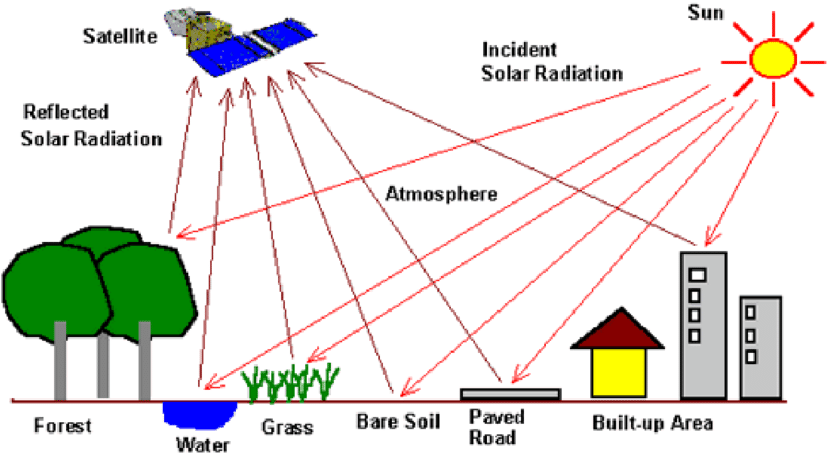
\includegraphics[height=8cm,keepaspectratio=true,clip=true]{imagenes/MarcoTeorico/teledeteccion.png}
  \caption{Sensado Remoto. Navarrete, Edison, Laubacher, Gerard}\label{Fig:teledeteccion}
\end{figure}

\subsubsection{Tipos de Sensores}
\begin{itemize}
\item \textbf{sensores pasivos}: son aquellos que reciben las señales emitidas naturalmente que fueron reflejadas por los objetos. Estas señales son a partir de la radiación solar natural. Este tipo de sensores son  usados mayormente en aplicaciones de evaluación de recursos naturales. Ejemplo: ASTER, MODIS, VIIRS, LandSat.

\item \textbf{sensores activos}: son aquellos que emiten radiación dirigida hacia un objetivo especifico, esta radiación reflejada del objeto es detectada y medida por el sensor. Ejemplo: Radar, Sonar.
\end{itemize}

\subsubsection{Espectro electromagnético}

El espectro electromagnético se denomina al conjunto de todas las longitudes de onda \citep{chuvieco}. Las ondas electromagnéticas cubren una amplia gama de frecuencias o de longitudes de ondas y pueden clasificarse según su principal fuente de producción. 
Las regiones utilizadas para la observación remota de la tierra son:
\begin{itemize}
\item Espectro visible (0.4 - 0.7 µm): rango de frecuencias del ojo humano; máxima radiación solar. Subdividido en tres bandas: Rojo (0.6 - 0.7 µm), Verde (0.5 - 0.6 µm) y Azul (0.4 - 0.5 µm).

\item Infrarrojo cercano (0.7 - 1.1 µm): denominado IR fotográfico o reflejado; energía solar que reflejan los cuerpos. Comportamiento similar al espectro visible.

\item Infrarrojo medio (1.1 – 8 µm): se entremezclan radiación solar y emisión; la atmósfera afecta sensiblemente: aprovechado para medir concentraciones de vapor de agua, ozono, aerosoles, etc.

\item Infrarrojo térmico (8 - 14 µm): radiaciones emitidas por los propios cuerpos; se puede determinar la Temperatura de un cuerpo (IRtérmico). Se puede disponer de imágenes a cualquier hora del día.

\item Microondas (1mm-1m): Interés creciente de la Teledetección en esta banda; las perturbaciones atmosféricas son menores y es transparente a las nubes. Se suelen utilizar sensores activos. 

\end{itemize}

\begin{figure}[H] \centering
  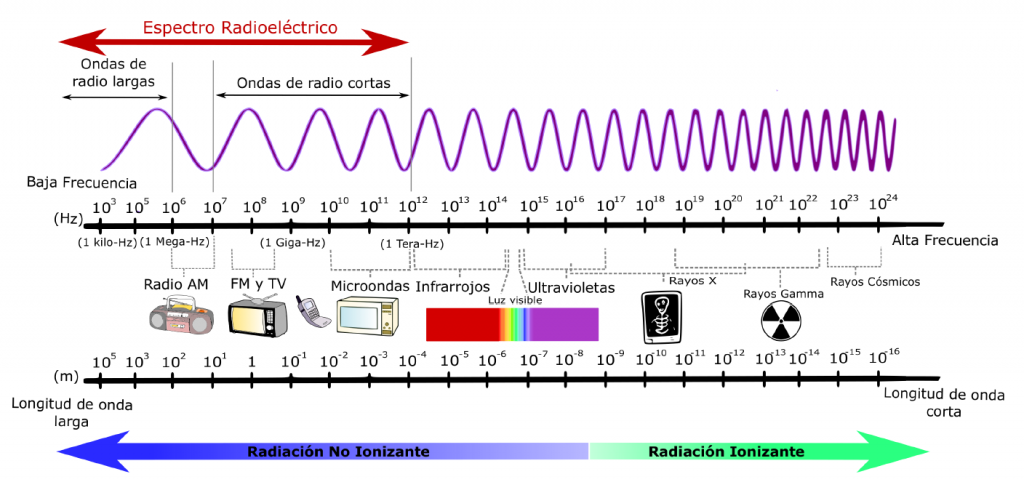
\includegraphics[height=8cm,keepaspectratio=true,clip=true]{imagenes/MarcoTeorico/espectro-electro.png}
  \caption{Espectro electromagnético \citep{https://iie.fing.edu.uy/proyectos/esopo/eem/}}\label{Fig:espectro-electromagnetico}
\end{figure}


\subsubsection{Resolución}
Unas de las características de los sensores son el tipo de imagen que proporciona; estas características vienen definidas por el timpo de resolución. Estas resoluciones la podemos definir de la siguiente manera:

\begin{itemize}
\item \textbf{Resolución Espacial}: distancia que corresponde a la unidad mínima de información incluida en un píxel. A menor tamaño de píxel mayor sera la resolución espacial, esto quiere decir que el sensor tendrá mayor detalle de los objetos.

\begin{figure}[H] \centering
  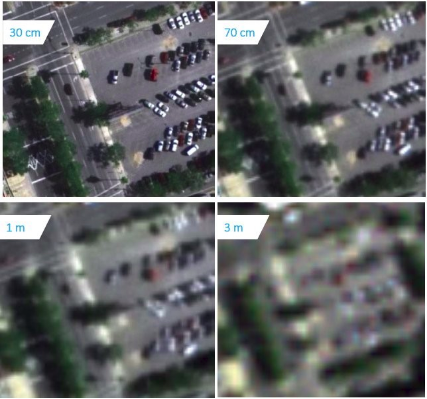
\includegraphics[height=8cm,keepaspectratio=true,clip=true]{imagenes/MarcoTeorico/resolucion.png}
  \caption{Resolución espacial \citep{https://iie.fing.edu.uy/proyectos/esopo/eem/}}\label{Fig:resolucion-esp}
\end{figure}

\item \textbf{Resolución Espectral}: la resolución espectral especifica el numero y la anchura de las badas espectrales que puede ser discrimidadas por el sensor.
\begin{figure}[H] \centering
  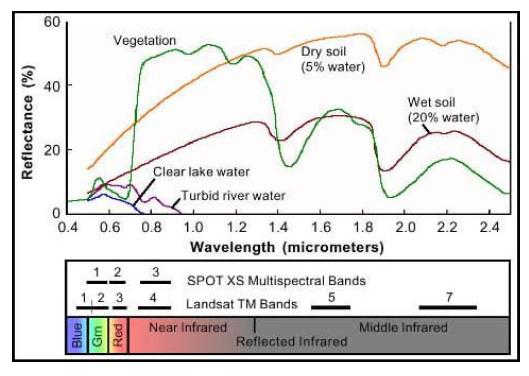
\includegraphics[height=8cm,keepaspectratio=true,clip=true]{imagenes/MarcoTeorico/resolucion_espectral.jpg}
  \caption{Resolución espectral \citep{http://laotraopinion.net/wp-content/uploads/poder-de-resolucion-espectral.jpg}}\label{Fig:resolucion-espectral}
\end{figure}

\item \textbf{Resolución Radiometrica}: indica el numero de bits utilizados para expresar los datos recogidos por el sensor. Mayormente cuando es mas grande el número de niveles mayor es el detalle con la cual se podrá expresar dicha información. Ejemplo los sensores Landsat (5 y 7) utilizan 8 bits lo que da 2**8= 256 niveles de energía que pueden ser captados.
\begin{figure}[H] \centering
  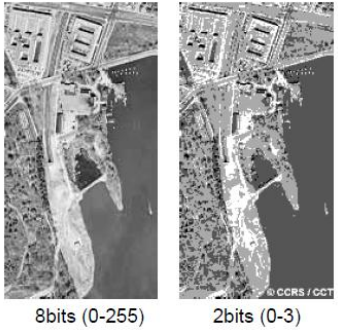
\includegraphics[height=8cm,keepaspectratio=true,clip=true]{imagenes/MarcoTeorico/resolucion_radiometrica.png}
  \caption{Resolución radiometrica}\label{Fig:resolucion-radiometrica}
\end{figure}

\item \textbf{Resolución temporal}: es el tiempo necesario que tarda el satélite en volver a visitar la misma zona de la Tierra; es decir la periodicidad con la que éste adquiere la misma imagen. Este ciclo de cobertura esta en función de el tipo de orbita de la plataforma así como del sensor. Alta resolución temporal (< 1 día - 3 días), media resolución temporal (4 - 16 días), baja resolución temporal (> 16 días).

\end{itemize}

\subsubsection{Imagen Satelital}
Una imagen satelital esta compuesta por diferentes matrices de las cuales cada celda representa un píxel; la dimensiones de este depende del tipo de resolución espacial como se mencionó anteriormente. Los sensores almacenan la raciación electromagnetica proveniente de distintas coberturas y las almacena en el píxel de acuerdo a los intervalos de onda correspondiente de cada sensor. Esta energia electromagnética se representa en cada píxel por un valor digital llamado Nivel Digital (ND), la cantidad de ND que se podrá representar depende de la resolución radiometrica.

La asignación de colores más conocido por los usuarios es el \textit{falso color} (R=Red (rojo); G=Green (verde); B=Blue (azul)), la cual asigna el color azul a la banda del verde, el color verde a la banda del rojo y el color rojo a la banda del infrarrojo cercano. 

La información obtenida de diferentes combinaciones de bandas depende del objeto de estudio que se esta llevando a cabo.

%https://acolita.com/wp-content/uploads/2018/01/Teledeteccion_espacial_ArcGeek.pdf
%https://mundosigs.wordpress.com/2016/03/07/que-son-los-sensores-remotos/
%https://www.slideshare.net/noldinn/fundamentos-deteledeteccionemiliochuvieco

\section{Aprendizaje Automático}

\subsection{Machine Learning}
\ac{ml} como se mencionó en la primera sección, es una rama de la inteligencia artificial que tiene como objetivo desarrollar técnicas que ayuden a las computadoras a aprender determinado comportamiento, generalizando, a partir de los datos de entrada. Un algoritmo de \ac{ml} es aquel que permite aprender determinado comportamiento a partir de los datos. \ac{ml} nos permite abordar tareas que son muy difíciles de resolver con programas escritos y diseñados por seres humanos.

"Se dice que un programa de computadora aprende de la experiencia E con respecto a algun tipo de tareas T y la medida de rendimiento P, si su desempeño en tareas en T, medido por P, mejora con la experiencia E." \citep{Tom michell}

Existen una gran cantidad de problemas que caen dentro de este tipo de rama, de las cuales podemos nombrar:

\begin{itemize}
\item \textit{Problemas de Regresión}: Este tipo de problema se pide que la computadora prediga un valor numérico dada alguna entrada. Los ejemplos que podemos citar son: fijar el precio de una casa a partir de las característica de la misma (cantidad de habitaciones, baños, etc), predecir el valor de la bolsa a partir del comportamiento de la bolsa en el tiempo pasado, entre otros.

\begin{figure}[H] \centering
  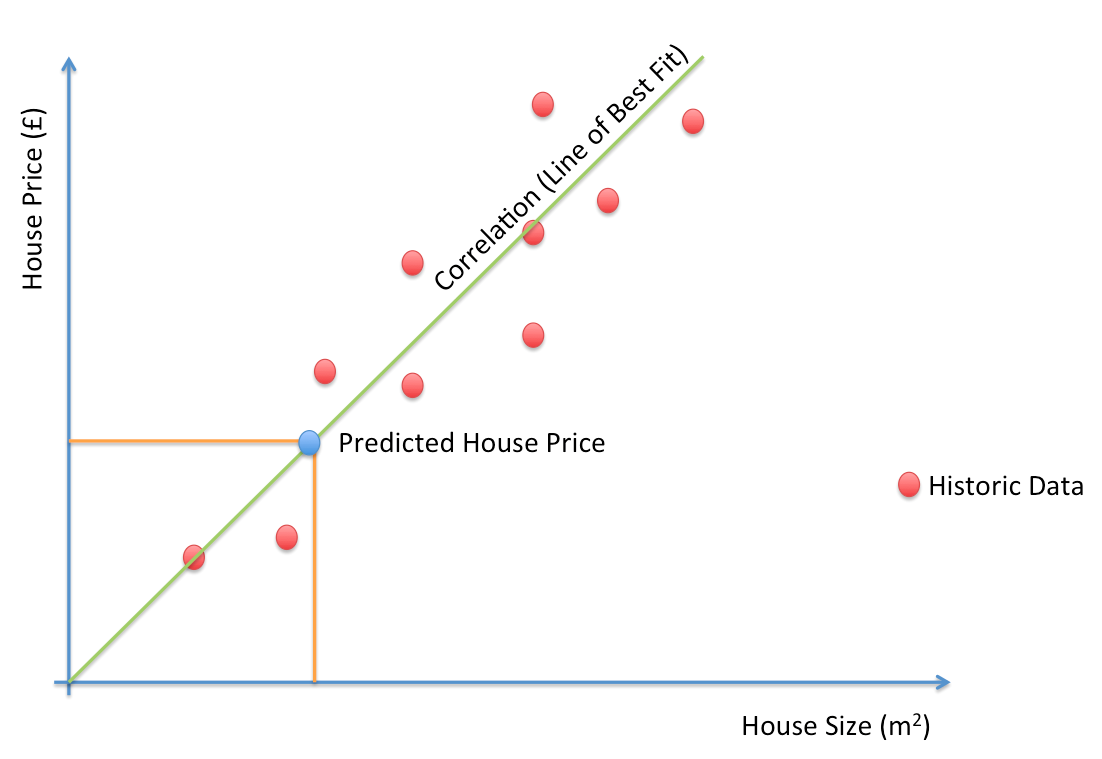
\includegraphics[height=8cm,keepaspectratio=true,clip=true]{imagenes/MarcoTeorico/regression_linear.png}
  \caption{Ejemplo Regresión (precio de una casa)}\label{Fig:regression}
\end{figure}

\item \textit{Problemas de Clasificación}: En un problema de clasificación, estamos tratando de predecir los resultados en una
salida discreta. En otras palabras, estamos tratando de asignar variables de entrada en categorías discretas. Algunos de los ejemplos son: clasificar perros o gatos determinando a que clase pertenece la imagen, evaluar si un email pertenece a la categoría "spam" o "no spam", entre otros.

\begin{figure}[H] \centering
  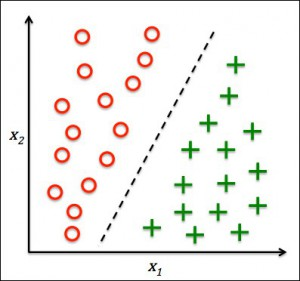
\includegraphics[height=8cm,keepaspectratio=true,clip=true]{imagenes/MarcoTeorico/classification.jpg}
  \caption{Ejemplo Clasificación}\label{Fig:clasificacion}
\end{figure}


\item \textit{Problemas de Aprendizaje no supervisado}: El aprendizaje no supervisado nos permite abordar los problemas con
poca o ninguna idea de cómo deben ser nuestros resultados. Podemos derivar la estructura de los datos donde no necesariamente conocemos el efecto de las variables. Podemos derivar esta estructura agrupando los datos basados en relaciones entre las variables en los datos. Con el aprendizaje no supervisado no hay una retroalimentación basada en los resultados de la predicción. El objetivo de problemas de aprendizaje no supervisados puede ser descubrir grupos de ejemplos similares dentro de los datos, donde se denomina agrupación (clustering), o determinar la distribución de datos dentro del espacio de entrada, conocida como estimación de densidad (density estimación), o proyectar los datos desde un espacio de nivel dimensional alto hasta dos o tres dimensiones con propósitos de visualización (Bishop, 2006).

\begin{figure}[H] \centering
  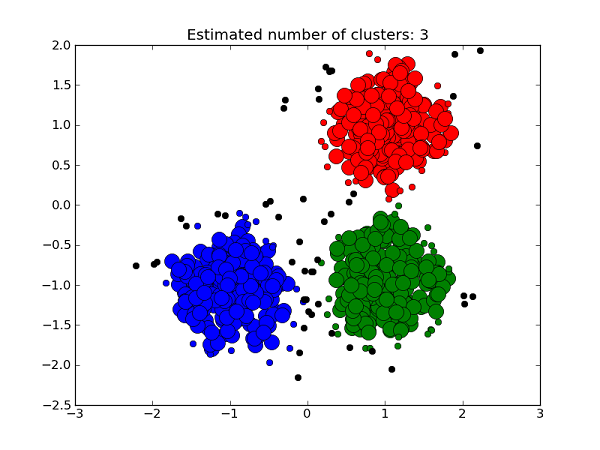
\includegraphics[height=8cm,keepaspectratio=true,clip=true]{imagenes/MarcoTeorico/claustering.png}
  \caption{Ejemplo aprendizaje no supervisado, claustering}\label{Fig:clauster}
\end{figure}
\end{itemize}

\subsubsection{Entrenamiento del modelo}
%https://docs.aws.amazon.com/es_es/machine-learning/latest/dg/training-ml-models.html
%clasificación supervisada metodos deduccion matematica
Entrenar un modelo de \ac{ml} consiste en proporcionar un conjunto de datos de entradas, datos de entrenamiento, de las cuales el algoritmo va a aprender. El algoritmo encuentra patrones en los datos proporcionados de entrada y genera un modelo que captura y generaliza dichos patrones para luego realizar predicciones sobre datos que no conoce.

Para poder entrenar un modelo necesitamos al menos tres cosas especificas:
\begin{enumerate}
\item \textbf{Datos de entrada}: determinar cuales son los ejemplos de entrada del algoritmo, el objetivo es crear un modelo que generalice los nuevos datos; para esto los datos de entrada deben ser representativo del mundo real. Por ejemplo para una tarea de clasificación entre perros y gatos los datos de entrada deben ser imágenes que pertenezcan a las categorías mencionadas; para resolver un problema de reconocimiento de voz los datos de entrada deben ser audios de personas hablando.

\item \textbf{Salida esperada}: para cada valor de entrada debemos etiquetar a que clase pertenece es decir, para un problema de clasificación entre perros y gatos debemos tener etiquetada cada imagen para saber a que clase pertenece la imagen; para un ejemplo de reconocimiento de voz cada audio debe tener una transcripción del mismo.

\item \textbf{Evaluación de las predicciones}: calcular y evaluar métricas con los resultados de la predicciones obtenidas por los modelo, es decir, determinar la distancia entre la salida esperada y los valores predichos.
\end{enumerate}

Como se desarrollo anteriormente el proceso de entrenamiento tiene: variables de entrada (x) y una variable de salida (Y); que a través de un algoritmo de aprendizaje obtenemos la siguiente relación entre estas variables como vemos a continuación.


\begin{eqnarray}
 f:X \longrightarrow Y\\
 \mbox{Training}:\qquad \{(x^i, y^i) \in X\; x\; Y \} _i=1...n\\
 \mbox{El objetivo es encontrar}\; f\; \mbox{tal que:}\qquad f(x)\approx y
\end{eqnarray}

Considerando el siguiente ejemplo, dada las cordenadas (x,y) como se muestra en la siguiente figura \ref{Fig: ejemplo-1}, se muestran dos clases, puntos de color negro y otra blanca.
\begin{figure}[H] \centering
  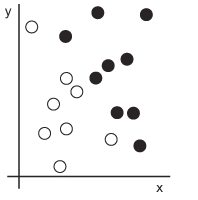
\includegraphics[height=4cm,keepaspectratio=true,clip=true]{imagenes/MarcoTeorico/sample.png}
  \caption{Ejemplo entrenamiento}\label{Fig:ejemplo-1}
\end{figure}

La idea principal de desarrollar un modelo; es crear un algoritmo que a partir de datos encuentre automáticamente una frontera, clasifique, por ejemplo encuentre una frontera entre los puntos negros y los puntos blancos.

Como se puede ver en la figura siguiente \ref{Fig:ejemplo-2}, se muestra la fontera de separación creada por el algoritmo entrenado.
\begin{figure}[H] \centering
  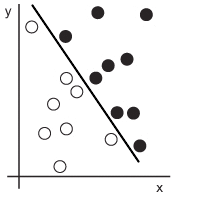
\includegraphics[height=4cm,keepaspectratio=true,clip=true]{imagenes/MarcoTeorico/sample-fit-1.png}
  \caption{Entrenamiento}\label{Fig:ejemplo-2}
\end{figure}

De esta manera cuando se pase un elemento que nunca vio puede determinar en cual de los dos espacios creado por el modelo cae este nuevo dato; en este caso estamos hablando en un algortimo de clasificación.

\subsubsection*{Ejemplo: Regresión Lineal}
%http://www.deeplearningbook.org/contents/ml.html
Una Regresión lineal es un claro ejemplo de un algoritmo de \ac{ml}; el objetivo es desarrollar un sistema que tome un vector $x \in \; $R$^n$, prediga el valor de un escalar $y \in \; $R$ $ como salida; la salida de una regresión lineal es una función lineal de la entrada.  Vamos a tomar como $\hat{y}$ el valor que nuestro modelo predice definido por:
\begin{equation}
\hat{y} = w^t * x
\end{equation}
donde $w \in \; $R$ $, siendo un vector de parámetros.
Los parámetros son valores que controlan el comportamiento del sistema,en este caso w  multiplicado por x (característica de cada datos de entrada), lo podemos ver como un conjunto de pesos que determinan como cada característica afecta a la predicción.

Si x esta multiplicado por un peso $w_i $ positivo, entonces el valor de esa característica aumenta nuestra predicción, de manera análoga si el valor $w_i $ es negativo esa característica x disminuye mi valor de predicción $\hat{y}$.
Como siguiente medida debemos medir la precisión de nuestro modelo, para realizar la medición de nuestro modelo debemos anteriormente haber separado el conjunto de datos en dos partes por un lado los datos de que se van a usar para realizar el entrenamiento y por otro los datos que serán utilizados para medir la precisión del modelo, llamado conjunto de test.

Una de las maneras de medir nuestra precisión del modelo con nuestro conjunto de test es computando el error cuadrado medio, dado por la siguiente ecuación:
\begin{equation}\label{eqn:mse} 
MSE_{test} = \frac{1}{n}\sum_{i}(\hat{y}^(test)- y^(test))^2
\end{equation}

Como se puede ver a partir del calculo anterior el error decremento a 0 cuando $\hat{y}$ es igual a $y$. Para entrenar un modelo de \ac{ml} necesitamos realizar un algoritmo que en cada iteración mejore los valores de los pesos de manera de reducir el error; en la sección siguiente se desarrollará mas en detalle.

Decimos que una hipótesis generaliza bien, cuando predice correctamente con entradas no conocidas.

\subsubsection{Función de Costo}
Existen diferentes maneras de que una algoritmo aprenda los parámetros de un modelo, este proceso de aprendizaje es posible minimizando la función de costo. Una función de costo es una medida del cuán erróneo es el modelo que estamos entrenando en términos a la capacidad de estimar la relación entre $X $ e $y $. Esto se lo puede expresar como la diferencia o distancia entre el valor predicho y el actual valor.

Como se menciono anteriormente el objetivo de un modelo de \ac{ml} es encontrar los valores que minimicen la función de costo.Una función de costo toma un conjunto de datos y retorna un valor llamado error costo (\textit{loss cost} su traducción en ingles). Existen diferentes tipos de funciones de costo que podemos usar; una de las mas comunes usada es \textbf{mean square error}, MSE, visto en \ref{eqn:mse}, en este caso determina la distancia o simplemente la diferencia entre el dato y el predictor $(x_i - y_i) $ ver figura: \ref{Fig:mse}.
\begin{figure}[H] \centering
  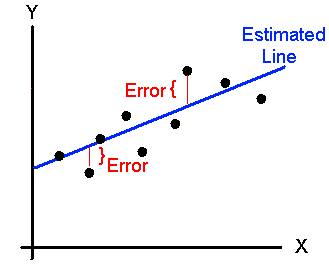
\includegraphics[height=4cm,keepaspectratio=true,clip=true]{imagenes/MarcoTeorico/mse-cost.png}
  \caption{Mean Square Error }\label{Fig:mse}
  %http://wiki.fast.ai/images/5/55/Linear_line_w_cost_function.png
\end{figure}

Dado un punto de datos $(x_i,y_i) $, donde $x_i $ es el conjunto de característica (por ejemplo pisos, dormitorios, etc) que el modelo usa para realizar la predicción, $y_i $ es la etiqueta del ejemplo (por ejemplo precio de la casa) e $y(x_i)$ es la la función de predicción; el error esta dado por la siguiente formula:
\begin{equation}\label{eqn:error-mse}
e = (y(x_i) - y_i)^2
\end{equation} 
A partir del calculo anterior podemos generalizar y tomar el promedio sobre todo los punto de datos de la siguiente manera:
\begin{equation}
MSE =  \frac{1}{n}\sum_{i}(y_i - y(x_i))^2
\end{equation}
% NOTA: SE DEBE PONER MAS FUNCIONES DE COSTO RMSE?

Existen en la actualidad diversas funciones de costo que nos permite calcular el error del modelo; entre ellas estan: Quadratic cost, Cross-entropy cost, Exponentional cost, Hellinger distance, Kullback–Leibler divergence, entre otras.

%https://stats.stackexchange.com/questions/154879/a-list-of-cost-functions-used-in-neural-networks-alongside-applications

\subsubsection{Algoritmos de Optimización} 
%https://hackernoon.com/gradient-descent-aynk-7cbe95a778da
%https://stxlearning.com/2018/03/25/optimizacion-deep-learning-y-complejidad-computacional/
En modelos de \ac{ml} debemos encontrar aquellos parámetros que minimizan la función de costo como se menciono previamente, este es un problema de optimización ya que si encontramos la solución podemos encontrar esos parámetros que disminuyen el error.

En la mayoría de los algoritmos de \ac{ml} deben aprender mas de un parámetro, en algunos casos hasta decenas de millones de parámetros; es por esto que todos los algoritmos  son métodos de optimización ya que se busca aprender los parámetros de manera eficiente. La estrategia mas típica para problemas de optimización son los llamados métodos de descenso; dentro de estos se encuentran: descenso de gradiente, descenso de gradiente estocástico y método de Newton Rawson de 2 orden.

\subsubsection*{Descenso de gradiente}\label{sub:gradient-desc}
Para encontrar el mínimo valor para grandes dimensiones de datos el algoritmo mas utilizado es el llamado \textbf{Descenso de Gradiente} (\textit{gradient descent} en ingles). El descenso de gradiente es un algoritmo de optimización que busca encontrar el mínimo local o global de una función convexa.  En \ac{ml} usamos descenso de gradiente para encontrar los parámetros de nuestro modelo que mejor definen nuestro conjunto de entrenamiento.

Este algoritmo permite que el modelo aprenda el gradiente o la dirección que el modelo debe seguir para reducir el error; en cada iteración gradualmente converge hacia un mínimo optimizando los valores $w_i $ que minimizan la función de costo. $$\min_{w} f(w)$$

Esto quiere decir que queremos encontrar los parámetros $w$ que minimicen la diferencia entre las salidas $Y$ y las producidas por el modelo dependiente de $w$. Entre menor  diferencia mejor aproximación a la salida $Y$. 

\begin{figure}[H] \centering
  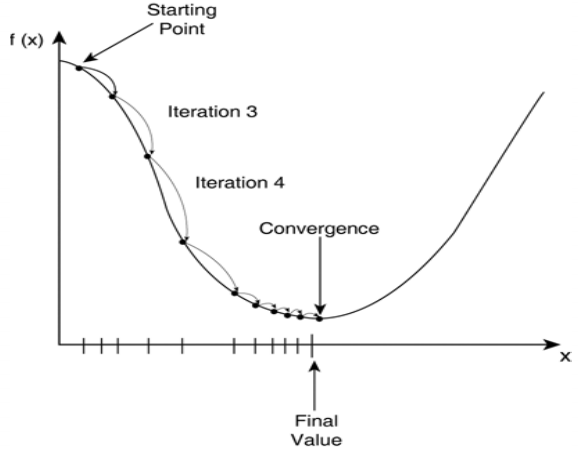
\includegraphics[height=6cm,keepaspectratio=true,clip=true]{imagenes/MarcoTeorico/gradient-descent.png}
  \caption{Gradient Descent }\label{Fig:gradient-descent}
\end{figure}


%Gradiente extraido de :https://www.cs.huji.ac.il/~shais/UnderstandingMachineLearning/understanding-machine-learning-theory-algorithms.pdf
El gradiente de una función diferenciable $ f: R^d \longrightarrow R $ en $\textbf{w}$, denotado $ \nabla f(w) $ vector de derivadas parciales de la función $f$ es decir:
\begin{equation}
\nabla f(x) = (\frac{\partial f(\textbf{w})}{\partial w[1]},....., \frac{\partial f(\textbf{w})}{\partial w[d]})
\end{equation}

Descenso de gradiente es un algoritmo iterativo; comenzamos con un valor inicial de $\textbf{w}$ (el valor 0 por ejemplo), luego en cada iteración damos un paso en la dirección negativa del gradiente en el punto actual. Es decir, el paso de actualización es:
\begin{equation}
\textbf{w}^{(t-1)} = \textbf{w}^{(t)} - n \nabla f(\textbf{w}^{(t)})
\end{equation}
En el cual $n > 0$, dado que el gradiente apunta a la dirección del mayor índice de $f$ alrededor $w^{(t)}$, el algoritmo va en sentido opuesto disminuyendo el valor de la función. Luego de T iteraciones se genera un vector promedio dado por: $ \hat{w} = \frac{1}{T} \sum_{t=1}^T w^{(t)}$; la salida también puede ser el vector con mayor  $ argmin_{t \in [T]} f(w^{(t)}) $.


En dónde $\hat{w}$ es una nueva posición de los parámetros que se acercan más al mínimo buscado, es decir que hacen que $f(w^{(t)})$ aproxime mejor a $Y$ . Existen diversas variantes de descenso por gradiente como Batch gradient descent, Stochastic gradient descent y Mini-batch gradient descent.

% PONEMOS BACKPROPAGATION, LEARNING RATE
%http://ruder.io/optimizing-gradient-descent/
%https://turing.iimas.unam.mx/~ivanvladimir/posts/gradient_descent/

\subsubsection{Validación de Modelos}
%Validación de Modelos (overfitting, underfitting)
Para determinar la persición de un modelo necesitamos realizar un evaluación de cuan bien nuestro modelo puede generalizar los datos y lograr una predicción correcta dado un valor de entrada desconocido. Las técnicas de validación en \ac{ml} son usadas para obtener esa tasa de error en el modelo.

Antes de evaluar nuestro modelo debemos separar nuestro datos en: \textit{datos de entrenamiento} y \textit{datos de test}; en la mayoria de los casos se suele realizar una separación del conjunto de datos total en porcentajes de 60/40, 70/30 o 80/20 para entrenamiento y test.

Una de las principales causas de validar nuestro modelo son obtener resultados erroneos en la predicción; esta causa esta dada por dos términos muy importante que debemos tener en cuenta: \textbf{ overfitting y underfitting}. \textit{\textbf{Overfitting}} y \textit{\textbf{underfitting}} son dos grandes problemas en \ac{ml} que influye en la performance del modelo. 

\subsubsection*{Overfitting}
Este concepto en \ac{ml} hace referencia al sobreentrenamiento del modelo. El overfitting ocurre cuando un modelo aprende en detalle junto al ruido en los datos de entrenamiento afectando negativamente el rendimiento del modelo en los nuevos datos a predecir. Esto significa que el ruido o las fluctuaciones aleatorias en los datos de entrenamiento son aprendidos como conceptos por el modelo. El problema es que estos conceptos no se aplican a los nuevos datos e impactan negativamente en la capacidad de generalización de los modelos.

\subsubsection*{Underfitting}
Como parte opuesta al overfitting esta el  underfitting; este concepto hace referencia a aquellos modelos que no pueden generalizar nuevos datos de entrenamiento de manera correcta. Mayormente en problemas de underfitting se necesita mayores características de los datos para la construcción de los modelos.

\begin{figure}[h]
 \centering
  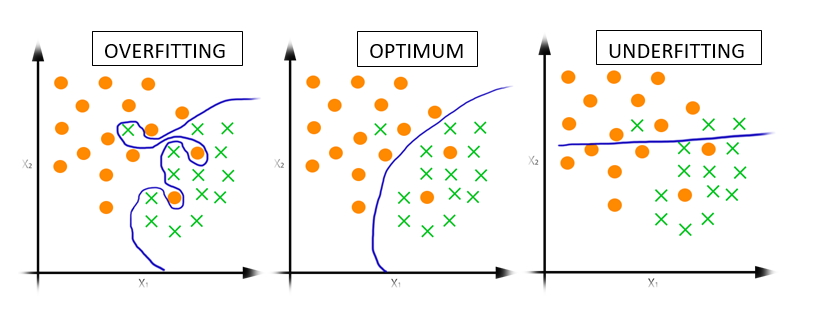
\includegraphics[height=5cm,keepaspectratio=true,clip=true]{imagenes/Logos/OverFUnderF.png}
  \caption{Ejemplo de overfitting (izquierda), modelo óptimo (centro) y underfitting (derecha)}
	\label{Fig: overUnder}
\end{figure}


Existen diferentes técnicas para validar la robustez de nuestro modelo y evitar los problemas mencionados anteriormente, una de ellas es por  \textit{validación cruzada} (cross validation en ingles). La validación cruzada es una técnica que evalúa los resultados de un análisis estadístico y garantiza de que sean independientes de la partición de los datos de entrenamiento y prueba. 

Hay diversos tipos de validación cruzada, de las cuales podemos nombrar:

\begin{enumerate}

\item \textbf{K-Fold Cross Validation}: consiste en dividir el conjunto de datos en \textit{k} subconjuntos. Exite un $k-1 $ valor que es el de validación, es decir, se toma uno de los subconjunto y se los utiliza como validación y el resto comom entrenamiento.  Este proceso se repite durante $k $ iteraciones con cada uno de los subconjunto de dato de validación. Para finalizar se utilizar aquel subconjunto de datos que posea mayor generalidad.
\begin{figure}[H]
 \centering
  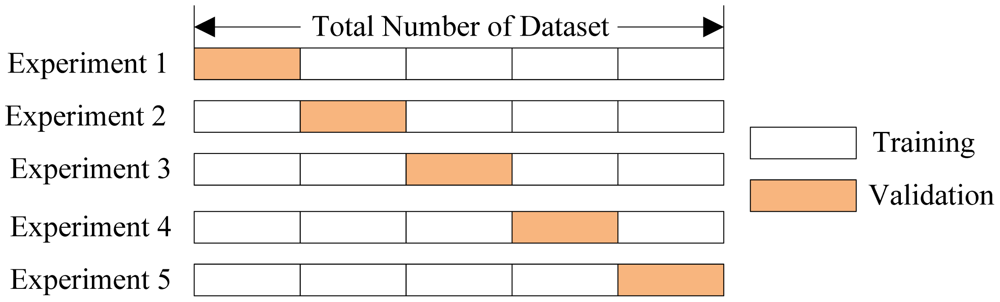
\includegraphics[height=5cm,keepaspectratio=true,clip=true]{imagenes/Logos/crossvalidat.png}
  \caption{Validación cruzada para k=5\\(Adaptado de:{http: //goo.gl/Dp85h3})}
	\label{Fig: crossvalidation}
\end{figure}

\item \textbf{Leave-One-Out Cross-Validation (LOOCV)}: Es un caso particular de validación cruzada, tomamos todos los datos que poseemos y utilizamos solo uno del subconjunto para validar. La ventaja de este metodo es que usamos todo los datos para realizar el entrenamiento.

\begin{figure}[H]
 \centering
  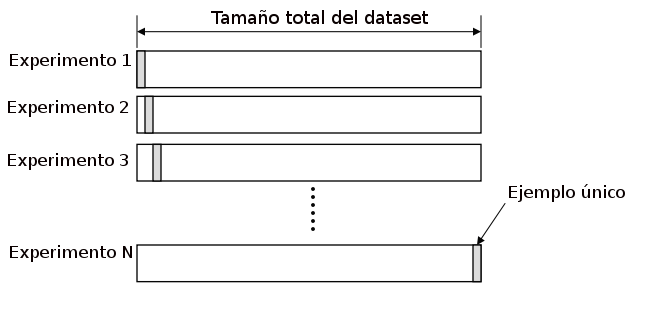
\includegraphics[height=5cm,keepaspectratio=true,clip=true]{imagenes/MarcoTeorico/cross-validation-LOOCV.png}
  \caption{Leave-One-Out Cross-Validation (LOOCV)}
	\label{Fig: crossvalidation-LOOCV}
\end{figure}

\item \textbf{Random Subsampling}: En esta técnica, se eligen aleatoriamente múltiples conjuntos de validación y se combinan para formar un conjunto de datos de prueba. Los datos restantes forman el conjunto de datos de entrenamiento.

\begin{figure}[H]
 \centering
  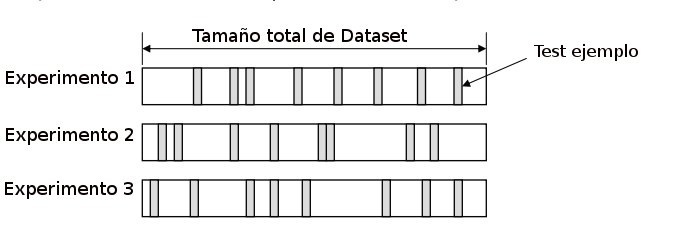
\includegraphics[height=5cm,keepaspectratio=true,clip=true]{imagenes/MarcoTeorico/cross-validation-random.png}
  \caption{Random Subsampling}
	\label{Fig: random-Subsampling}
\end{figure}

\end{enumerate}


%IMPORTANTE: https://sebastianraschka.com/pdf/manuscripts/model-eval.pdf
%https://dzone.com/articles/machine-learning-validation-techniques

\subsection{Computer Vision}

\subsection{Ajuste de Modelos}

\subsection{Redes Convolucionales}

\subsection{Regions Proposal}

\subsection{Clasificadores}







